% Question  ##################################################################################################################
\section{Question 5}\label{ssec:pt2q5}

\textbf{You are working in an organisation providing Machine Learning consultancy. As an organisation you have access to internal private data, however you wish to start selling Machine Learning models, as a service, trained on, but without sharing, this private data. With the availability of blockchain you decide to make this business model work via smart contracts. As a proof of concept you are asked to:}

% END Question  ##############################################################################################################

% Question (i) ###############################################################################################################

\subsection{Q5 (i)}\label{sssec:pt2q5i}
\textbf{Utilize the standard Iris data set (assuming it’s internal/private data) and create a simple logistic regression model to create a classification model (utilize only 80\% of the data for training).}

% END Question (i) ###########################################################################################################

% Question (ii) ##############################################################################################################

\subsection{Q5 (ii)}\label{sssec:pt2q5ii}

\textbf{Define and deploy a smart contract. As the owner of the contract, you are allowed to upload (or update) the trained model parameters from the off-chain ML training software on the smart contract. }

% END Question (ii) ##########################################################################################################

% Question (iii) #############################################################################################################

\subsection{Q5 (iii)}\label{sssec:pt2q5iii}

\textbf{Simulate a typical organisation client, assuming that the client has the remaining 20\% unseen data (hence assuming that this 20\% of the data is public). The client has his own off-chain client program that is allowed to request the trained model parameters from the smart contract. For each request}

\begin{itemize}
  \item (a) The client receives the logistic regression trained parameters.
  \item (b) The client is automatically charged 0.01 ether from his account and transferred to the organisation account. 
\end{itemize}

% END Question (iii) #########################################################################################################

% Question (iv) ##############################################################################################################

\subsection{Q5 (iv)}\label{sssec:pt2q5iv}

\textbf{Once the client receives the trained model parameters, the client applies the logistic regression parameters received from the smart contract to his local untrained model and performs out-of-sample testing on the remaining 20\% of the data set. }

% END Question (iv) ###########################################################################################################

% Present (a) #################################################################################################################

\subsection{Present (a)}\label{sssec:pt2q5a}

\textbf{A description of the approach and technologies used.}

\noindent
Code for this task is in \textit{‘src/solidity/ml\_consultancy\_truffle’}. Inside the location provided there is a folder called \textit{‘contracts’} were the smart contract called ‘MlConsultancy.sol’ is used to manage this use case. Also, there is a folder called \textit{‘python’} which has two scripts called ‘ml\_consultancy.py’ (holds classes for Client and Operator) and another script called 'prototype.py' which is used to showcase the prototype. 

\noindent
The following approach was taken to create a prototype for this task. First off, a new contract was created called ‘MlConsultancy.sol’ and this contract inherits from ‘Ownable.sol’ provided by OpenZepplin. The ‘Ownable.sol’ gives us basic functionality to check that the owner of the contract can access a specific function (with the use of a modifier in the contract) and other functionalities such as transferring ownership. Such contract was slightly modified, so the owner address is set to be payable since we need the payable keyword to send funds to the owner as described in the question.

\noindent
After creating the contract two structs were written for specific purposes as shown in Fig.~\ref{fig:model_sol_1}. The first struct ‘Model’ holds details about the model. This contract was written with the assumption that the operator/organization can upload multiple models which clients can pay for (makes the proof of concept more similar to a real-world application). From the comments it is easy to understand what the variables inside the struct are used for. The other struct ‘ModelWeights’ is used to hold information about the weights for a specific available model. Comments in the code explains what the variables inside the struct are used for. It is important to note that the variable called ‘nDecimals’ is used to keep track of where to put the decimal point, since the weights and intercept are saved as integer values on the network (EVM does not support floating point numbers). This variable will be utilised by the client to convert the integer values to floating points. 

\begin{figure}[H]
\centering
  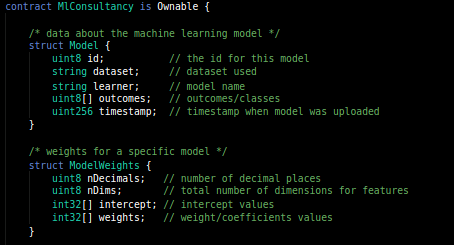
\includegraphics[scale = .75]{imgs/model_sol_1.png}
  \caption{Two structs used in the 'MlConsultancy.sol' contract.}
  \label{fig:model_sol_1}
\end{figure}

\noindent
After creating the structs described the variables and constructor shown in Fig.~\ref{fig:model_sol_2} were written to the contract. The ‘SERVICE\_COST’ is the cost (0.01 ether) for which the client needs to pay to access the weights as specified in the question. For the purposes of this proof of concept the number of different models which can be uploaded to the contract/chain is capped to 255, which is why the constant ‘maxModels’ was specified. The ‘modelWeights’ variable holds a reference to the ‘ModelWeight’ struct given the model id (the same id in the ‘Model’ struct) is used as a key. ‘clientAccess’ mapping is a used to hold a reference for which access and to what model a specific address/client has. Finally, the ‘modelCount’ variable is set, which holds a reference to how many models are available in the contract. When the contract is deploying and the constructor is called we want that the ‘modelCount’ is set to 0.

\begin{figure}[H]
\centering
  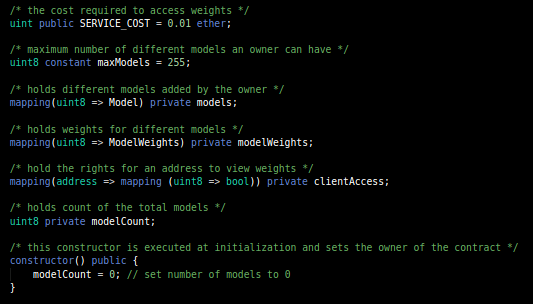
\includegraphics[scale = .75]{imgs/model_sol_2.png}
  \caption{Variables and constructor in the 'MlConsultancy.sol' contract.}
  \label{fig:model_sol_2}
\end{figure}

\noindent
Two simple functions then were written, which basically return the service cost and the number of models available as shown in Fig.~\ref{fig:model_sol_3}. 

\begin{figure}[H]
\centering
  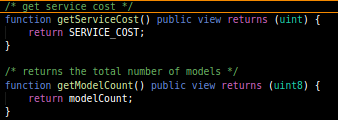
\includegraphics[scale = .75]{imgs/model_sol_3.png}
  \caption{Get cost and get model count functions in the 'MlConsultancy.sol' contract.}
  \label{fig:model_sol_3}
\end{figure}

\noindent
Another function was created called ‘getModelDetails’ and as the name implies it gets the details for a specific model. The model id must be passed as a parameter and this function like the other two functions above can be accessed by any address. This will return the model id, the name of the dataset used to train this model, the name of the machine learning model used, the different labels which can be outputted for the problem it was trained for and the timestamp when the model details were uploaded. Such function gives potential client/customers or even existing customers to view available models which can be sold by the organization. This function is shown in Fig.~\ref{fig:model_sol_4}. 

\begin{figure}[H]
\centering
  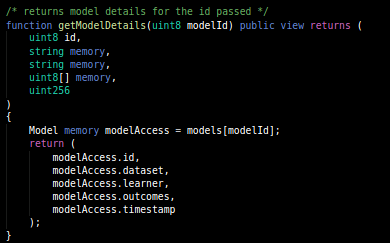
\includegraphics[scale = .75]{imgs/model_sol_4.png}
  \caption{Get model details function in the 'MlConsultancy.sol' contract.}
  \label{fig:model_sol_4}
\end{figure}

\noindent
The next function which was written is the ‘addModel’ function which allows the owner (the one who deployed the contract) to add new models along with the weights to the contract. In this case the owner of the contract (organization providing the service) can access this function and this is why there is a ‘onlyOwner()’ modifier to restrict others from adding models to this contract. This function is shown in Fig.~\ref{fig:model_sol_5}. 

\begin{figure}[H]
\centering
  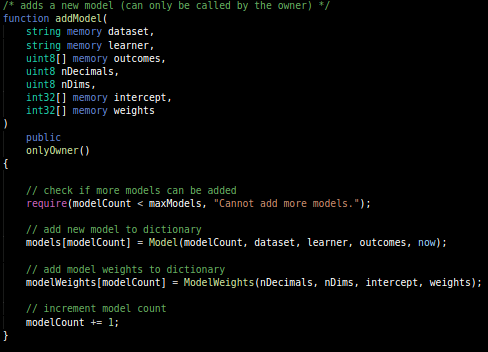
\includegraphics[scale = .75]{imgs/model_sol_5.png}
  \caption{Add model function in the 'MlConsultancy.sol' contract.}
  \label{fig:model_sol_5}
\end{figure}

\noindent
The following parameters must be specified to add the model to the contract; the name of the dataset used to train the model, the name of the machine learning model, the outcomes which can be outputted by the model, the place where to put the decimal point to (when converting back integers to floats), the number of dimensions/features in the dataset, the intercept learned by the model and finally the weights learned by the model.  Once these parameters are passed a struct ‘Model’ is created and added to the ‘models’ mapping and a ‘ModelWeights’ struct is created and added to the ‘modelWeights’ mapping. The id for both mapping is the ‘modelCount’ and at the end of this function this value is incremented by 1. 

\noindent
Following this function, the ‘updateModel’ was created which enables the organizer to update the weights and intercept of an existing model as described in the question. This function is shown in Fig.~\ref{fig:model_sol_6}. 

\begin{figure}[H]
\centering
  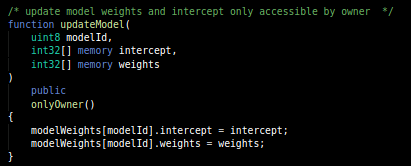
\includegraphics[scale = .75]{imgs/model_sol_6.png}
  \caption{Update model function in the 'MlConsultancy.sol' contract.}
  \label{fig:model_sol_6}
\end{figure}

\noindent
The next function which was written is quite important for this task, the ‘payService’ allows clients to pay for the service to be able to access the model weights for the model which they paid for. This function is shown in Fig.~\ref{fig:model_sol_7}. The client who transacts this function must send the specified value of 0.01 ether and the model id must be specified. In this function the funds are automatically transferred to the organizer as specified in the question. A reference in the ‘clientAccess’ mapping is taken where it is noted (setting bool to true), that an address has access to the weights for the model id which was specified (passed as a parameter).

\begin{figure}[H]
\centering
  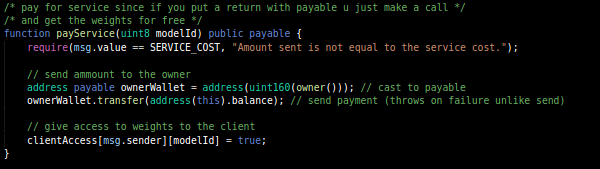
\includegraphics[scale = .75]{imgs/model_sol_7.png}
  \caption{Pay for service function in the 'MlConsultancy.sol' contract.}
  \label{fig:model_sol_7}
\end{figure}

\noindent
The final function is the ‘getWeights’ which allows clients who paid for a specific model to access its weights. This function is shown in Fig.~\ref{fig:model_sol_8}. The client requesting the weights must specify the model id and the weights are returned only if the client previously paid by calling the ’payService’ function (the require part does this validation by checking that the value in the mapping ‘clientAccess’ is set to true). The following information is then sent to the client if everything is valid; the outcomes for the model, the point where to put the decimal point, the number of features, the intercept which was learnt and the weights which was learnt. That concludes the approach taken from the contract side.             

\begin{figure}[H]
\centering
  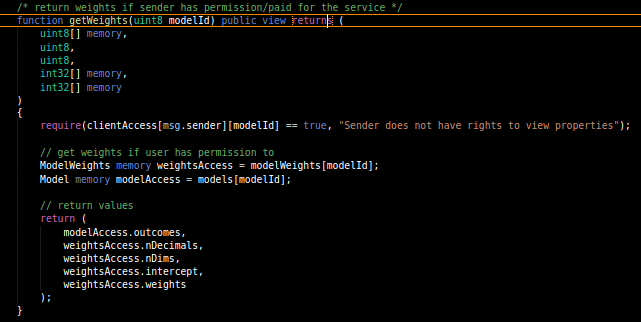
\includegraphics[scale = .75]{imgs/model_sol_8.png}
  \caption{Get weights function in the 'MlConsultancy.sol' contract.}
  \label{fig:model_sol_8}
\end{figure}

\noindent
Two new python classes were created in the ‘ml\_consutlancy.py’, one for the client which is called ‘Client’ and the other is called ‘Operator’ which is used by the organization. Both classes inherit from another created class called ‘Service’ which basically provides common functions between the two to interact with the contract. In this section the most important functions in the classes will be described, as for the other functions everything is well documented and can be viewed from the script. 

\begin{figure}[H]
\centering
  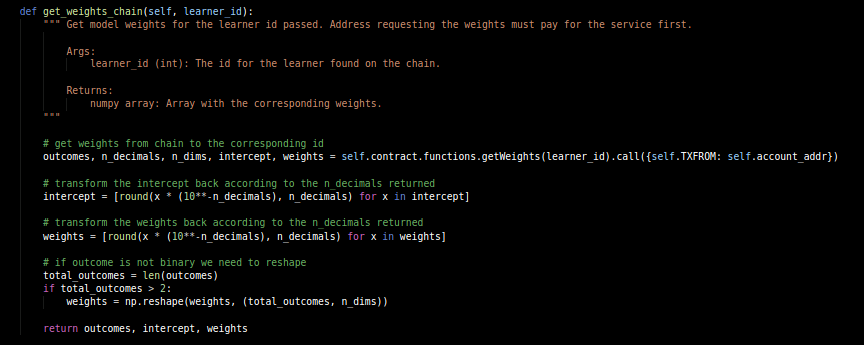
\includegraphics[scale = .55]{imgs/model_sol_py_1.png}
  \caption{Get weights from the chain in the 'Service' class in the 'mlconsultancy.py'.}
  \label{fig:model_sol_py_1}
\end{figure}

\noindent
The function ‘get\_weights\_chain’ as shown in Fig.~\ref{fig:model_sol_py_1} is found the ‘Service’ class which is a base class for the other two classes mentioned above. This allows for the instance to fetch the weight for a specific model with a specific id if this instance have paid for the service. In our use case this will be utilised by the ‘Client’ class, but it was decided to put this function in the base class. As shown in the function both the ‘weights’ and ‘intercept’ are transformed back to floating point numbers using the ‘n\_decimals’ sent back from the chain. Also, if the outcome for the specified model is not binary the ‘weights’ array is transformed accordingly. 

\noindent
The second function in the python script which will be described is the ‘set\_weights\_chain’ as shown in Fig.~\ref{fig:model_sol_py_2} and this too reside in the ‘Service’ base class. This will be utilised by the client to set the weights for a local model to the weights received from the chain. The main reasons why these two functions were written in the base class although these are mostly utilised by the ‘Client’, is that it may be the case that the service might want to reload a model with the weights found on the chain. This function takes two parameters, the first parameter ‘learner\_id’ is used to retrieve the local model from the collection of local models and the second parameter ‘chain\_learner\_id’ is used to retrieve the weights from a model which is found on the chain. First the function calls the ‘get\_weights\_chain’ function which was described previously and apply the returned values to the local model. 

\begin{figure}[H]
\centering
  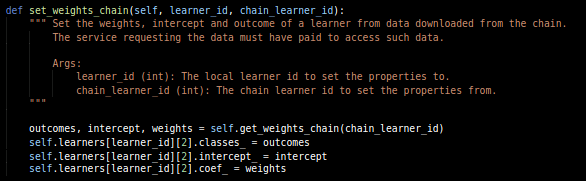
\includegraphics[scale = .65]{imgs/model_sol_py_2.png}
  \caption{Set weights from the chain in the 'Service' class in the 'mlconsultancy.py'.}
  \label{fig:model_sol_py_2}
\end{figure}

\noindent
Now we will look at the important functions found in the ‘Operator’ class. The first function ‘upload\_model\_chain’ as shown in Fig.~\ref{fig:model_sol_py_3} allows the operator/organization (the ones who deployed the contract) to upload a model’s weight from a local model in the collection to the chain. Before data could be uploaded on the chain it must be processed using the function ‘\_\_prep\_for\_upload’ as shown in Fig.~\ref{fig:model_sol_py_4}. In this function the necessary values are gathered and the floating-point values in both the ‘weights’ and ‘intercept’ values are transformed to integers for reasons described above. Once the data is processed the function adds this information on the chain for clients to pay for. The final function is called ‘update\_model\_chain’ which lets the operator update the weights on the chain for a specific model. Only the weights can be updated as shown in Fig.~\ref{fig:model_sol_py_3}. 

\begin{figure}[H]
\centering
  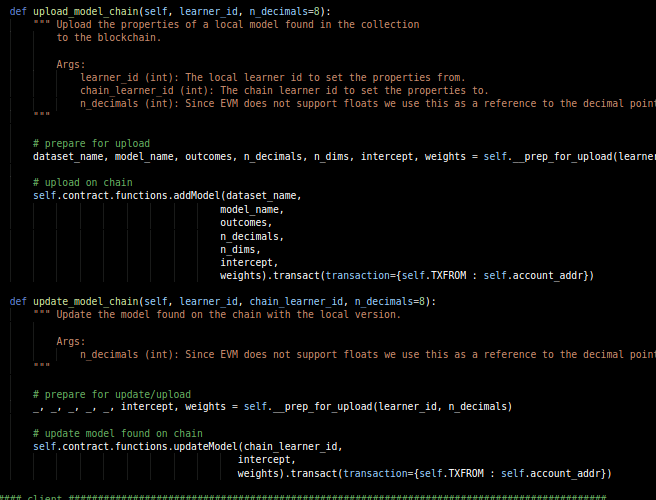
\includegraphics[scale = .52]{imgs/model_sol_py_3.png}
  \caption{Add and Update model functions in the 'Operator' class in the 'mlconsultancy.py'.}
  \label{fig:model_sol_py_3}
\end{figure}

\begin{figure}[H]
\centering
  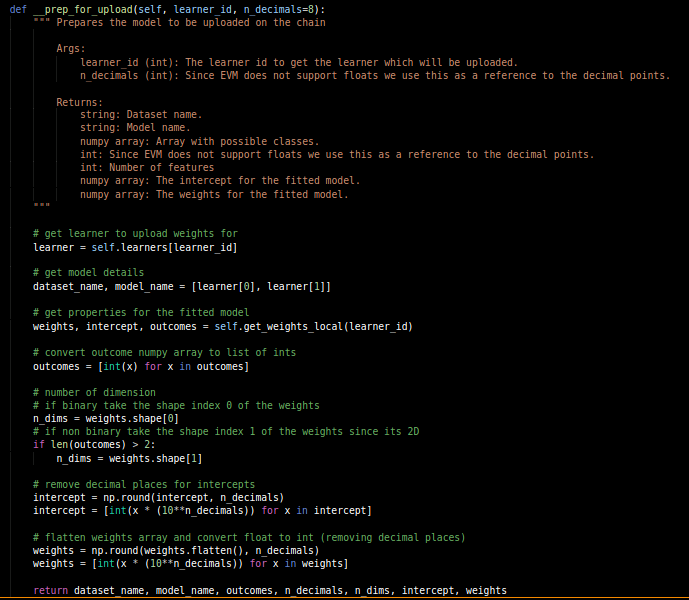
\includegraphics[scale = .53]{imgs/model_sol_py_4.png}
  \caption{Prepare data for upload function in the 'Operator' class in the 'mlconsultancy.py'.}
  \label{fig:model_sol_py_4}
\end{figure}

\noindent
The final function described ‘pay\_service\_chain’ as shown in Fig.~\ref{fig:model_sol_py_5} is found in the ‘Client’ class. Such function allows for a client instance to pay for a specific model found on the chain. The model id must be passed, and this refers to the id for the model which is on the chain.  

\begin{figure}[H]
\centering
  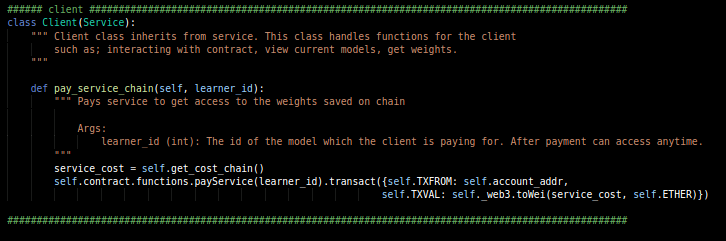
\includegraphics[scale = .65]{imgs/model_sol_py_5.png}
  \caption{Pay for service function in the 'Client' class in the 'mlconsultancy.py'.}
  \label{fig:model_sol_py_5}
\end{figure}

\noindent
Now we will look at the step by step process used to showcase the proof of concept. Code for this task can be found in the python script called ‘prototype.py’. The iris dataset was loaded from ‘sklearn.datasets’ and it was split into 80\% which will be utilized by the ‘Operator’ and 20\% which will be utilized  by the ‘Client’. A new instance of the ‘Operator’ was instantiated, and the contract was deployed from this address using the function ‘deploy\_contract’. The path for the compiled contract was passed as a parameter to this function. After doing so a ‘LogisticRegression’ model was added to the local collection of models in the ‘Operator’ instance using the ‘add\_learner’ function. This local model was then fitted using the ‘fit\_learner’ function. Weights for the fitted model were then uploaded to the chain using the ‘upload\_model\_chain’ function. 

\noindent
An instance for ‘Client’ was instantiated. The ‘get\_details\_chain’ function was called to view the available models which are offered by the consultancy (simulating the real-world environment). The model which was previously uploaded by the ‘Operator’ is shown in the list.  A local model was added to the Client’s collection of local models which reflects the model which the Client intends to pay for (a Logistic Regression Model). The client pays for the service to view the weights for the selected model by calling the ‘pay\_service\_chain’ function. Before and after this call both the client and operator balance were printed to test that the transfer is being made. The client retrieves the weights it paid for from the chain and set these weights to the untrained local model by calling the ‘set\_weights\_chain’ function.

\noindent
Using the 20\% of data found on the client side the ‘predict\_learner’ function was called, and the accuracy score was printed. Now we tested the model update function in the ‘Operator’ class. To do so the penalty for the local model in the operator’s collection was changed to ‘L1’ by calling the ‘set\_params\_learner’ function. The local model was then refitted and updated using the respective functions ‘fit\_learner’ and ‘update\_model\_chain’. The client reupdates the weights by re-querying the chain using the ‘set\_weights\_chain’ function and the accuracy score with the new weights was noted.

\noindent 
Technologies used in the process:

\begin{itemize}
  \item \textbf{Node.js:} To use the package manager ‘npm’ provided by Node.js to install JavaScript packages used in this task.
  \item \textbf{Truffle:} Installed using ‘npm’. This was used to compile the contract which was used in this task. The contract could have been compiled using ‘py-solc’ from python but there was no support for solidity version greater or equal to 0.5. The solidity compiler could also have been used for this process but preferred to utilise truffle. 
  \item \textbf{Ganache-cli:} Installed using ‘npm’, which is a command line interface for ganache. This allowed us to deploy the contract in a development/test environment. 
  \item \textbf{Web3.py:} Installed using ‘pip’ which is a python library to interact with the network. This is a python wrapper of the Web3.js implementation. 
  \item \textbf{OpenZepplin:} Installed using ‘npm’, a package which offers readily available contracts and interfaces. This was specifically installed to use the ‘Ownable.sol’ contract. 
\end{itemize}

\noindent
As we described our approach for the proof of concept, we would like to add some comments about this implementation. Since data in the Ethereum network is found on every full node, someone can find ways to read these weights found on the chain by not paying for the service at all. An approach to mitigate such risk is to encrypt the weights being uploaded by the consultancy agency. Once a client pays for the service the keys are sent via another means and the client can decrypt the information, but this solution reverts to having trust in a third party. Up till now there is now way to store secrets on the Ethereum chain. Another solution could be to use ‘Codius’, which provide a decentralized application layer which handles the use of secrets, but this project is in its early stages and it is very limited in functionality (also bugs are present). 

% END Present (a) ##############################################################################################################

% Present (b) #################################################################################################################

\subsection{Present (b)}\label{sssec:pt2q5a}

\textbf{Source code of the smart contract, code that handles the ML model training and upload of model parameters on smart contract, and client application (for the latter, showing both the code requesting the parameters and also the out-of-sample testing/results).}

\noindent
As described previous all the code used in this task can be found in:

\noindent
\textit{‘src/solidity/ml\_consultancy\_truffle’}

\noindent
The source code for the smart contract can be found in the location specified under the folder \textit{‘contracts’} and it is named as ‘MlConsultancy.sol’. 

\noindent
The code that handles the ML model training and upload of model parameters on smart contract can be found under the folder \textit{‘python’} in the ‘ml\_consultancy.py’ script (described in the previous question). The code for the interaction between the client application is then showcased in the ‘prototype.py’ script which is found in the same folder. Below are some figures showing the interaction and the results in the proof of concept (interactions were previously described in detail in the previous answer). 

\noindent
Fig.~\ref{fig:prototype_1} shows the code which handles the machine learning model training and the upload for the parameters. Fig.~\ref{fig:prototype_2} shows the interaction between the client and the smart contract and in Fig.~\ref{fig:prototype_3} the final outputs are shown. 


\begin{figure}[H]
\centering
  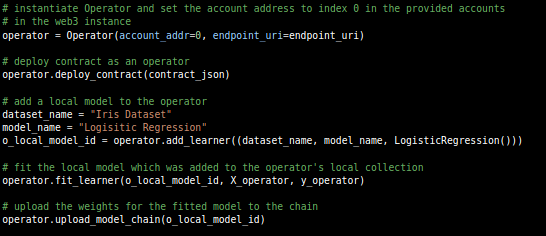
\includegraphics[scale = .65]{imgs/prototype_1.png}
  \caption{Code which handles the machine learning model training and the upload for the parameters in 'prototype.py'.}
  \label{fig:prototype_1}
\end{figure}

\begin{figure}[H]
\centering
  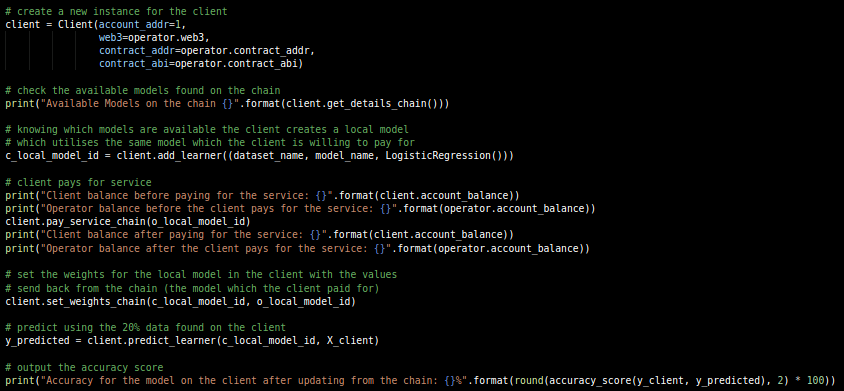
\includegraphics[scale = .55]{imgs/prototype_2.png}
  \caption{Interaction between the client and the smart contract (requesting weights) in 'prototype.py'.}
  \label{fig:prototype_2}
\end{figure}

\begin{figure}[H]
\centering
  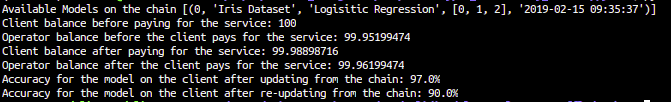
\includegraphics[scale = .65]{imgs/prototype_3.png}
  \caption{Final output produced by the 'prototype.py' script.}
  \label{fig:prototype_3}
\end{figure}

% END Present (b) ##############################################################################################################
